\documentclass[reprint, amsmath, amssymb, aps, pra, nofootinbib]{revtex4-2}

% --- Основные пакеты ---
\usepackage[T2A]{fontenc}
\usepackage[utf8]{inputenc}
\usepackage[russian,english]{babel}

\usepackage{graphicx}
\graphicspath{{figures/}}
\usepackage{bm}

% hyperref в REVTeX лучше подключать с параметрами или использовать встроенный механизм
\usepackage[unicode, colorlinks=true, linkcolor=blue, citecolor=blue, urlcolor=blue]{hyperref}

\begin{document}

\title{3.6.1 Спектральный анализ электрических сигналов}

\author{Иван Рудко}
\email{rudko.ia@phystech.edu} 
\affiliation{Московский физико-технический университет, группа Б02-506}

\author{Ефим Сычев}
\email{sychev.ea@phystech.edu}
\affiliation{Московский физико-технический университет, группа Б02-506}

\date{\today}

\begin{abstract}
В работе исследованы спектры различных электрических сигналов с помощью цифрового осциллографа с функцией быстрого преобразования Фурье. Изучены спектры периодической последовательности прямоугольных импульсов, цугов, а также амплитудно-модулированных сигналов. Экспериментально проверены соотношения неопределенностей. Полученные результаты согласуются с теоретическими зависимостями.
\end{abstract}

\maketitle

% --- Основной текст ---
\section{Введение}
Спектральный анализ электрических сигналов играет важную роль в исследовании линейных систем, подчиняющихся принципу суперпозиции. Знание реакции системы на гармонический сигнал позволяет с помощью разложения Фурье определить её отклик на произвольное воздействие. 

В данной работе исследуются спектры сигналов различной формы и влияние параметров сигнала (длительности, периода повторения, частоты модуляции) на вид соответствующих спектров. Основной целью является экспериментальная проверка соотношений неопределенностей.

\section{Физические основы явления}

\subsection{Ряд Фурье и спектр сигнала}

Согласно теореме Фурье, любая периодическая функция может быть представлена в виде ряда гармонических функций с кратными частотами. Для функции $f(t)$ с периодом $T$ представление имеет вид:
\begin{equation}
f(t)=\frac{a_{0}}{2}+\sum_{n=1}^{\infty}a_{n}\cos(2\pi \nu_{n}t+\varphi_{n}),
\end{equation}
где $\nu_{n}=n\nu_{0}$ (при $\nu_{0}=1/T$) — частоты гармоник, $a_{n}$ — амплитуды, $\varphi_{n}$ — фазы. Совокупность всех частот $\nu_{n}$ и соответствующих им амплитуд $a_{n}$ называется спектром электрического сигнала.

При устремлении периода $T \to \infty$ спектр непериодического сигнала (например, одиночного импульса) становится непрерывным, а разложение в ряд Фурье переходит в интеграл Фурье.

В данной работе частотный анализ осуществляется с помощью алгоритма быстрого преобразования Фурье, который применяется к оцифрованному входящему сигналу. 

\subsection{Соотношения неопределенностей}

Между сигналом как функцией времени $f(t)$ и его спектром как функцией частоты $a(\nu)$ имеется универсальная взаимосвязь. Если у сигнала есть характерное время $\Delta t$ (например, длительность импульса $\tau$), то в спектре наблюдается характерный масштаб $\Delta \nu \sim 1/\Delta t$ (например, ширина спектра). 

Данная связь выражается соотношением неопределенностей:
\begin{equation}
\Delta \nu \cdot \Delta t \sim 1.
\end{equation}

Кроме того, для любого сигнала с периодом $T$ в спектре обязательно наблюдаются гармоники, расстояние между которыми строго равно $\delta \nu = 1/T$.


\section{Экспериментальная установка}

В состав экспериментальной установки входят генератор сигналов произвольной формы, цифровой осциллограф и компьютер. Выходной канал генератора соединен с измерительным каналом осциллографа, который подключен к ПК. Управление процессом измерений, визуализация исследуемых сигналов во времени и расчет их частотных спектров осуществляются с помощью программы PicoScope 6. 

Поскольку измерения проводились преимущественно однократно для каждой конфигурации сигнала, случайной погрешностью можно пренебречь. Оценка полной погрешности выполнялась на основе инструментальной погрешности цифрового осциллографа и ошибки отсчета курсорных измерений в программе.

\section{Ход работы}

\subsection{Исследование спектра периодической последовательности прямоугольных импульсов}

На генераторе была задана генерация периодической последовательности прямоугольных импульсов.
Исходные параметры сигнала были установлены следующими: частота повторения $\nu_{\text{повт}} = 1$ кГц (период $T = 1$ мс), длительность импульса $\tau = 50$ мкс. После стабилизации картины на экране осциллографа был зарегистрирован частотный спектр сигнала с использованием функции преобразования Фурье.

Для корректного отображения масштаб по горизонтальной оси (оси частот) был выбран порядка ожидаемой ширины спектра $\Delta\nu$, оцениваемой из соотношения неопределенностей: $ \Delta \nu \sim 1/\tau = 20 \, \text{кГц}. $ Масштаб по вертикальной оси подбирался так, чтобы спектральные линии не выходили за пределы экрана, за исключением нулевой гармоники ($\nu = 0$ Гц), отвечающей за уровень постоянного смещения. Спектр был отцентрирован и смещен к левому краю экрана для охвата максимального частотного диапазона.

В ходе эксперимента исследовалось изменение спектра при различных параметрах исходного сигнала. Регистрация проводилась при изменении частоты повторения $\nu_{\text{повт}}$ (при фиксированном $\tau$), а также при изменении длительности импульса $\tau$ (при фиксированном $\nu_{\text{повт}}$). Масштабы по осям частот и амплитуд поддерживались строго фиксированными. Полученные спектрограммы представлены на рис. \ref{fig:spectra}.

\begin{figure*}[t!]
    \centering
    \begin{minipage}{0.48\textwidth}
        \centering
        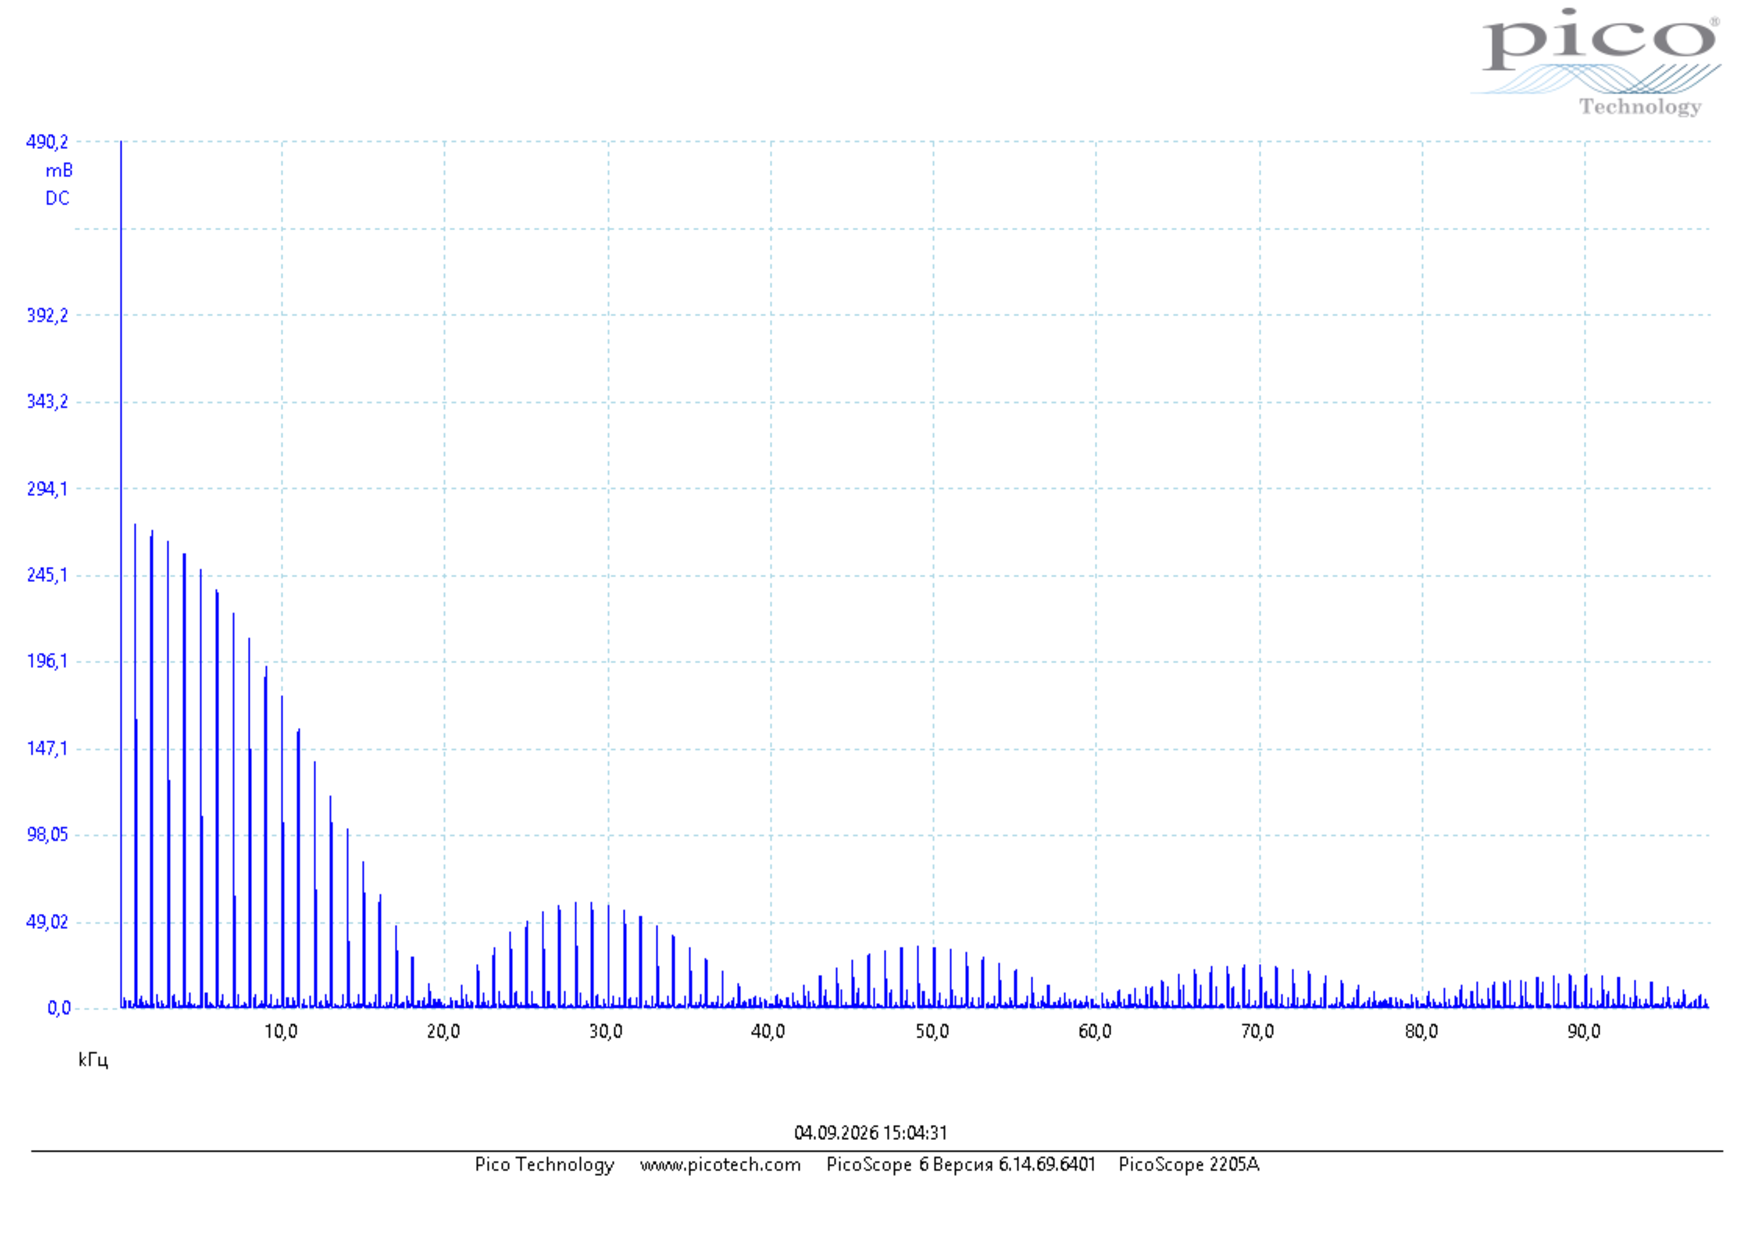
\includegraphics[width=\linewidth]{1kHz_50us.pdf}
        \vspace{-0.8em}
        
        \small а) $\nu_{\text{повт}} = 1$ кГц, $\tau = 50$ мкс (исходный)
        \vspace{4mm} 
    \end{minipage}\hfill
    \begin{minipage}{0.48\textwidth}
        \centering
        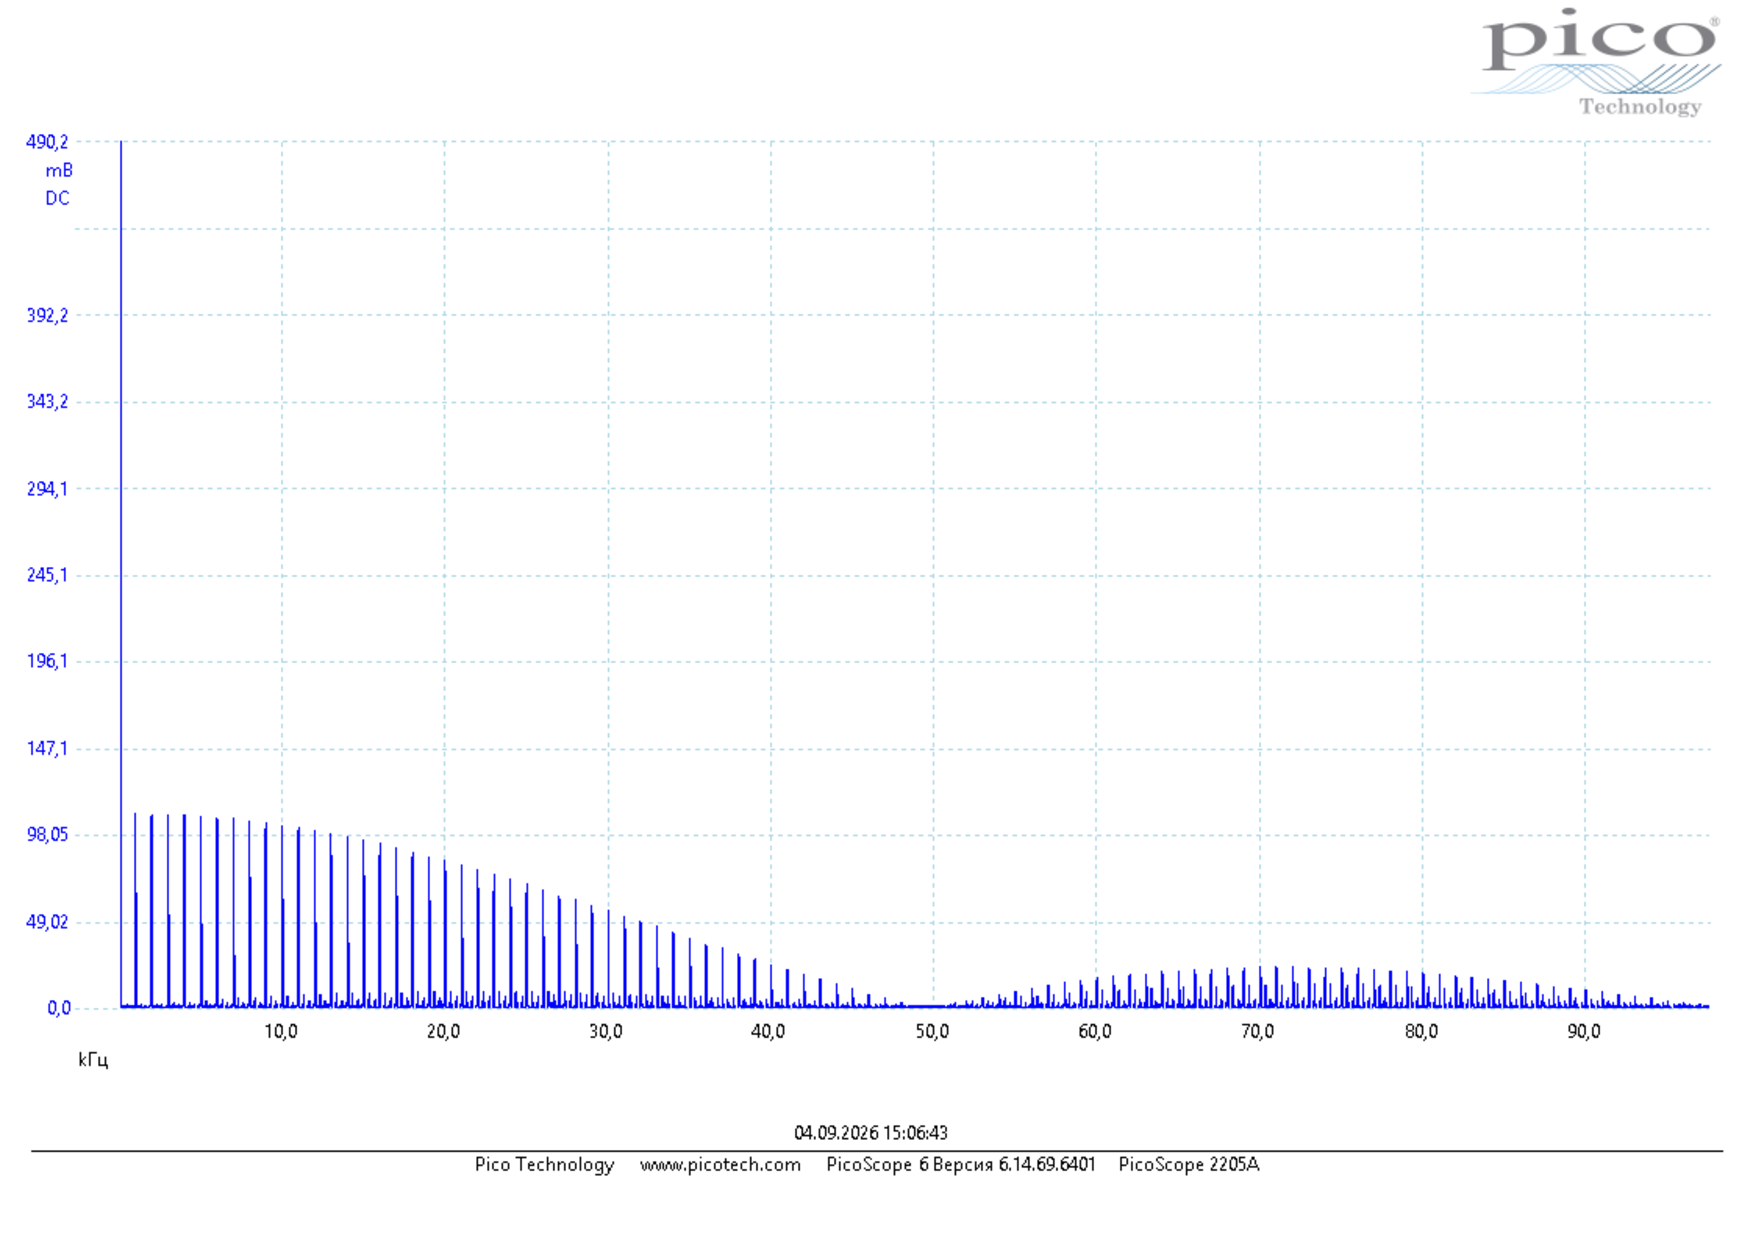
\includegraphics[width=\linewidth]{1kHz_20us.pdf}
        \vspace{-0.8em}
        
        \small б) $\nu_{\text{повт}} = 1$ кГц, $\tau = 20$ мкс
        \vspace{4mm}
    \end{minipage}
    
    \begin{minipage}{0.48\textwidth}
        \centering
        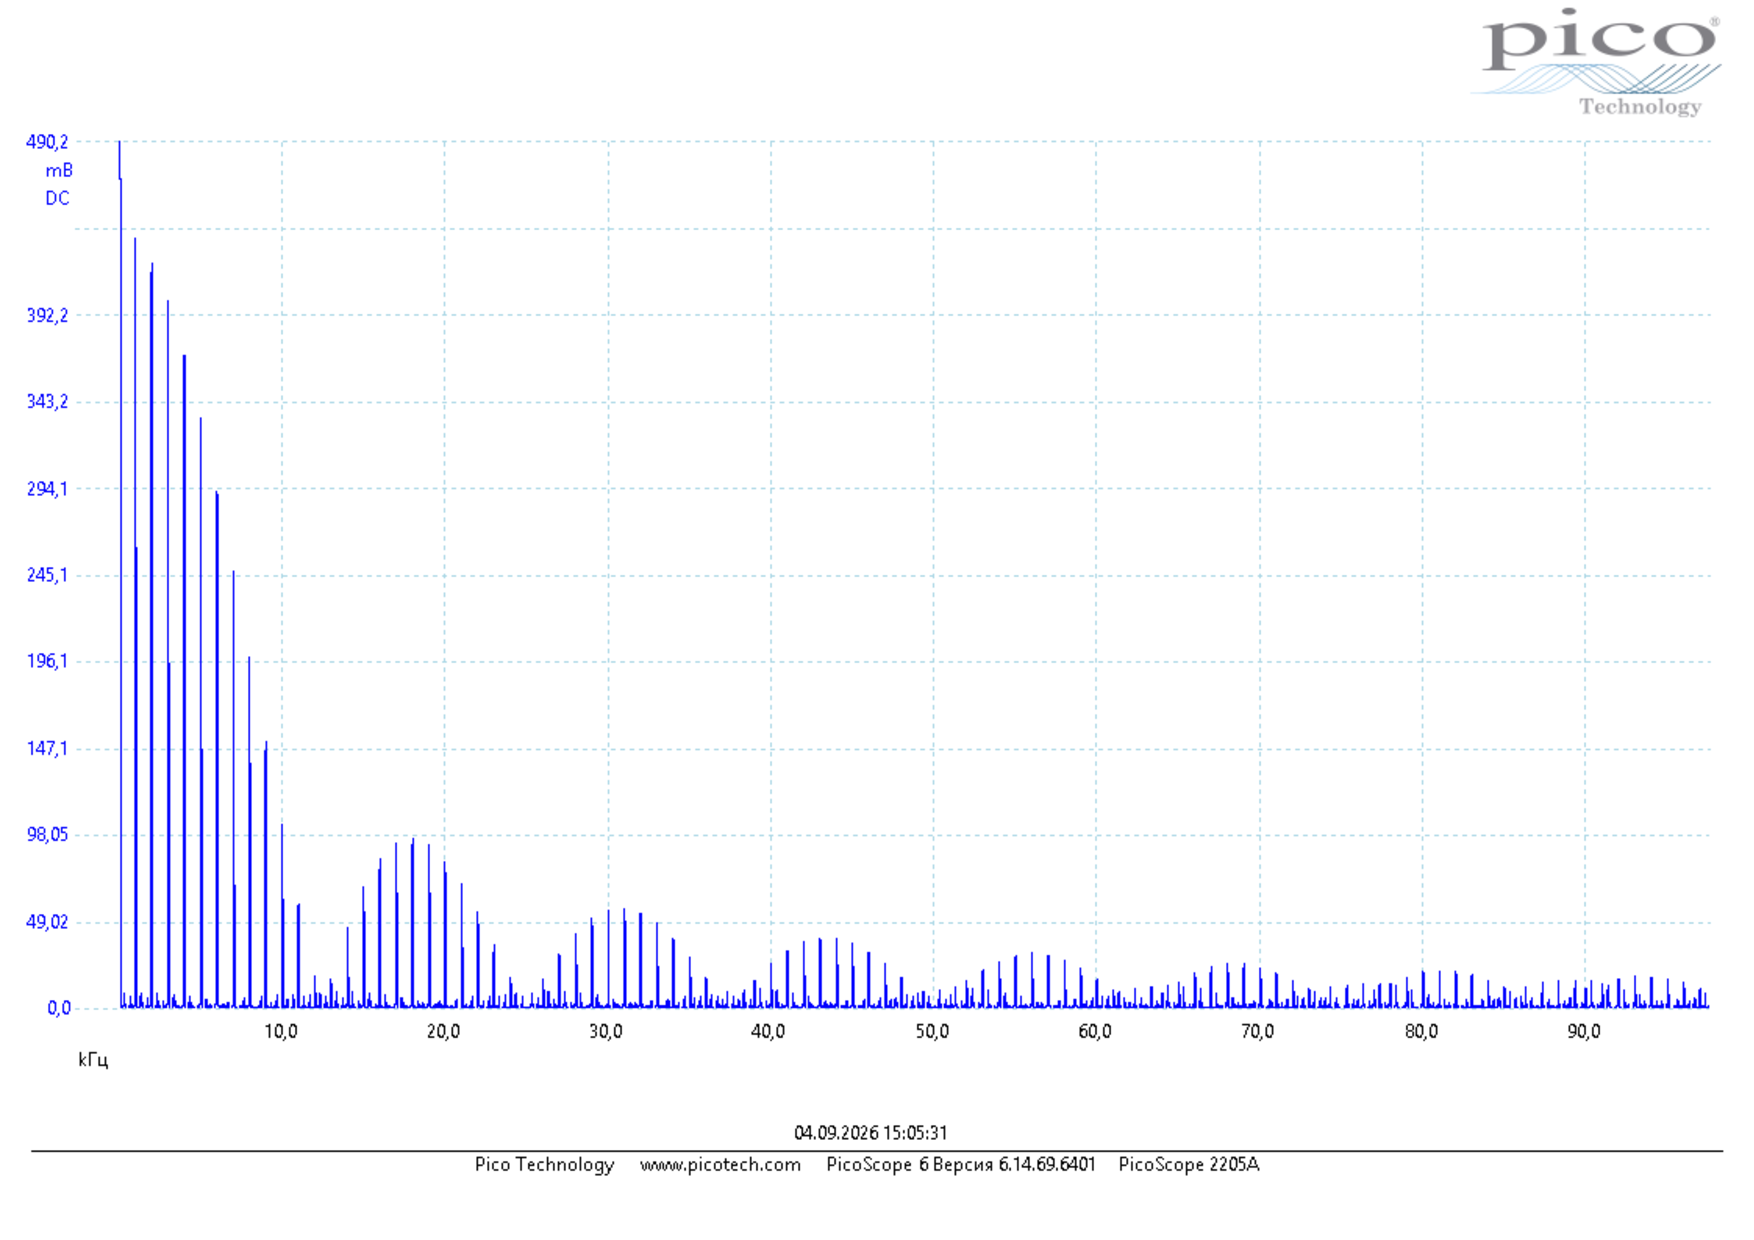
\includegraphics[width=\linewidth]{1kHz_80us.pdf}
        \vspace{-0.8em}
        
        \small в) $\nu_{\text{повт}} = 1$ кГц, $\tau = 80$ мкс
    \end{minipage}\hfill
    \begin{minipage}{0.48\textwidth}
        \centering
        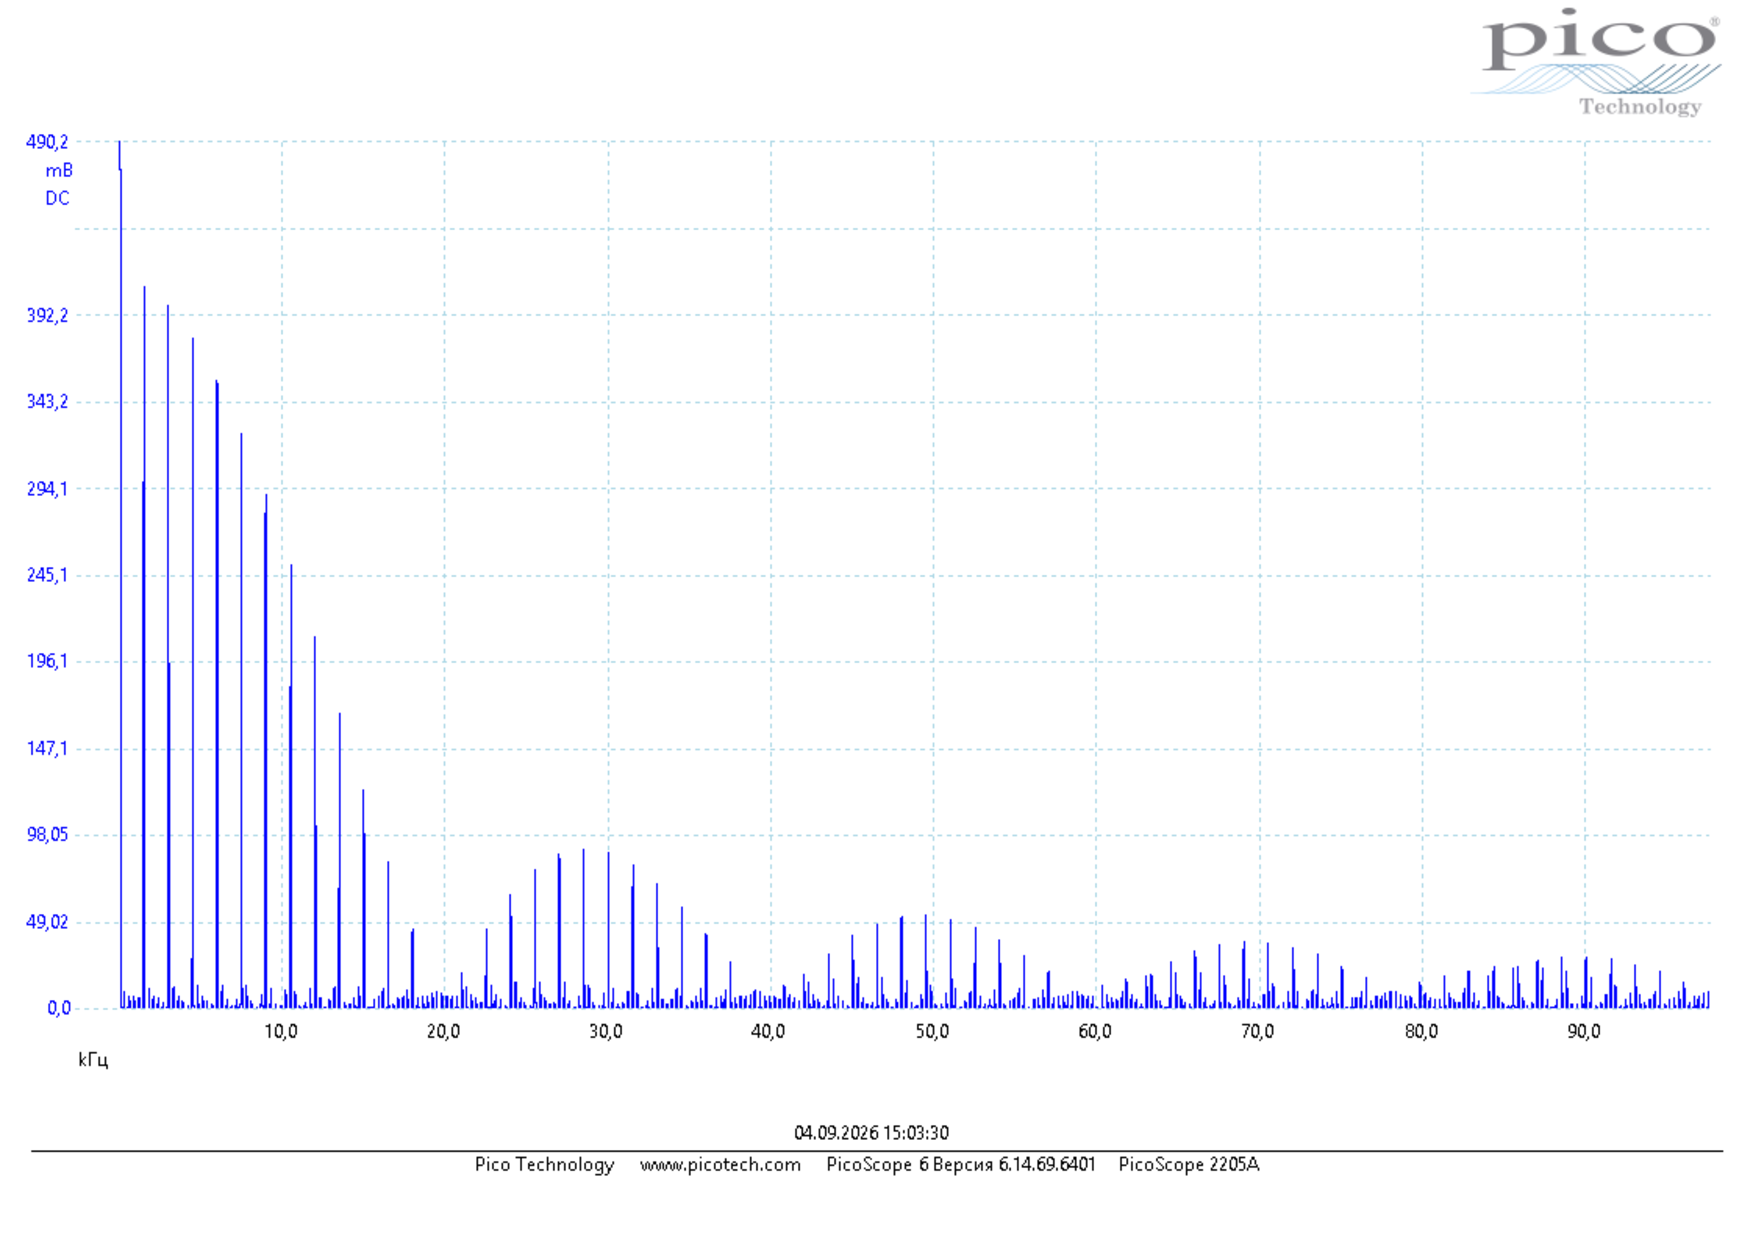
\includegraphics[width=\linewidth]{1.5kHz_50us.pdf}
        \vspace{-0.8em}
        
        \small г) $\nu_{\text{повт}} = 1.5$ кГц, $\tau = 50$ мкс
    \end{minipage}
    \caption{Спектры периодической последовательности прямоугольных импульсов: (а) при исходных параметрах; (б, в) при изменении длительности импульса; (г) при изменении частоты повторения. 
    \vspace{1em}}
    \label{fig:spectra}
\end{figure*}

Анализ полученных данных показывает, что при изменении длительности импульса $\tau$ (рис. \ref{fig:spectra} а, б, в) ширина огибающей спектра $\Delta\nu$ ведет себя обратно пропорционально $\tau$. При уменьшении длительности до 20 мкс спектр расширяется в $2.5$ раза, а при увеличении до 80 мкс — сужается в $1.6$ раз. Это наблюдение полностью согласуется с фундаментальным соотношением неопределенностей $\Delta\nu \sim 1/\tau$. 

Расстояние между спектральными линиями $\delta\nu$ в данной серии измерений остается постоянным ($\delta\nu = \nu_{\text{повт}} = 1.00 \pm 0.01$ кГц), поскольку оно определяется исключительно частотой повторения сигнала. С другой стороны, при увеличении частоты повторения $\nu_{\text{повт}}$ до 1.5 кГц (рис. \ref{fig:spectra} г) ширина огибающей спектра сохраняется идентичной исходной (рис. \ref{fig:spectra} а), однако расстояние между соседними гармониками пропорционально возрастает.

Для количественного анализа спектральных компонент были измерены частоты $\nu_n^{\text{эксп}}$ и амплитуды $|a_n|^{\text{эксп}}$ первых восьми гармоник сигнала. Измерения проводились при фиксированных параметрах генерации: частоте повторения $\nu_{\text{повт}} = 1$ кГц (период $T = 1$ мс) и длительности импульса $\tau = 50$ мкс.

Полученные экспериментальные значения сопоставлялись с теоретическими частотами $\nu_n^{\text{теор}} = n/T$ и расчетными амплитудами гармоник, определяемыми выражением:
\begin{equation}
    |a_n| = \frac{\tau}{T} \frac{|\sin(\pi \nu_n \tau)|}{\pi \nu_n \tau}.
\end{equation}

Поскольку абсолютные единицы измерения амплитуд на осциллографе произвольны, для корректного сопоставления использовались относительные величины $|a_n/a_1|$. Экспериментальные данные и результаты теоретических расчетов представлены в табл. \ref{tab:harmonics}. 

\begin{table}[ht!]
    \caption{Экспериментальные и теоретические параметры первых восьми гармоник спектра прямоугольных импульсов ($\nu_{\text{повт}} = 1$ кГц, $\tau = 50$ мкс).}
    \label{tab:harmonics}
    \centering
    \begin{ruledtabular}
    \begin{tabular}{cccccc}
        $n$ & $\nu_n^{\text{эксп}}$, Гц & $\nu_n^{\text{теор}}$, Гц & $|a_n|^{\text{эксп}}$, у.е. & $|a_n/a_1|^{\text{эксп}}$ & $|a_n/a_1|^{\text{теор}}$ \\
        \hline
        1 & $1000 \pm 10$ & 1000 & $274.3 \pm 0.3$ & $1.000$ & 1.000 \\
        2 & $2000 \pm 10$ & 2000 & $270.8 \pm 0.3$ & $0.987 \pm 0.002$ & 0.988 \\
        3 & $3000 \pm 10$ & 3000 & $265.2 \pm 0.3$ & $0.967 \pm 0.002$ & 0.967 \\
        4 & $4000 \pm 10$ & 4000 & $257.8 \pm 0.3$ & $0.940 \pm 0.002$ & 0.939 \\
        5 & $5000 \pm 10$ & 5000 & $248.3 \pm 0.3$ & $0.905 \pm 0.002$ & 0.904 \\
        6 & $6000 \pm 10$ & 6000 & $237.1 \pm 0.3$ & $0.864 \pm 0.002$ & 0.862 \\
        7 & $7000 \pm 10$ & 7000 & $224.2 \pm 0.3$ & $0.817 \pm 0.002$ & 0.814 \\
        8 & $8000 \pm 10$ & 8000 & $209.4 \pm 0.3$ & $0.763 \pm 0.002$ & 0.760 \\
    \end{tabular}
    \end{ruledtabular}
\end{table}

Как видно из представленных данных, измеренные частоты гармоник совпадают с расчетными значениями в пределах инструментальной погрешности. Относительные амплитуды монотонно убывают с ростом номера гармоники, при этом экспериментальные значения $|a_n/a_1|^{\text{эксп}}$ также хорошо согласуются с теоретическими предсказаниями $|a_n/a_1|^{\text{теор}}$ (отклонение не превышает 1.5\%).

Для всесторонней проверки соотношений неопределенностей были проведены две серии измерений, в которых параметры спектра исследовались в зависимости от временных характеристик сигнала. 

В первой серии период повторения прямоугольного сигнала фиксировался на значении $T = 1000$ мкс ($\nu_{\text{повт}} = 1$ кГц). Длительность импульса $\tau$ изменялась в диапазоне от $T/50$ до $T/5$, что соответствует значениям от 20 до 200 мкс. Измерялась полная ширина спектра $\Delta\nu$, определяемая как расстояние от центральной частоты $\nu = 0$ до первой гармоники с нулевой амплитудой $a_n \approx 0$. Результаты измерений представлены в табл. \ref{tab:width_tau}.

Во второй серии измерений фиксировалась длительность импульса $\tau = 100$ мкс, а период повторения $T$ изменялся в диапазоне от 400 до 5000 мкс. Для каждого значения $T$ измерялось расстояние $\delta\nu = \nu_{n+1} - \nu_n$ между соседними гармониками спектра. В случаях высокой плотности спектральных линий для снижения погрешности расстояние измерялось между $(n+m)$-й и $n$-й гармониками с последующим усреднением: $\delta\nu = (\nu_{n+m} - \nu_n)/m$. Данные измерений приведены в табл. \ref{tab:dist_T}.

\begin{table}[b!] 
    \caption{Зависимость ширины спектра $\Delta\nu$ от обратной длительности импульса $1/\tau$ при фиксированном периоде $T = 1$ мс. Инструментальная погрешность измерения ширины спектра составляет $\pm 0.1$ кГц, погрешность измерения обратной длительности импульса пренебрежимо мала.}
    \label{tab:width_tau}
    \centering
    \begin{ruledtabular}
    \begin{tabular}{ccc}
        $\tau$, мкс & $1/\tau$, кГц & $\Delta\nu_{\text{эксп}}$, кГц \\
        \hline
        20  & 50.00 & $50.0 \pm 0.1$ \\
        40  & 25.00 & $25.0 \pm 0.1$ \\
        60  & 16.67 & $16.9 \pm 0.1$ \\
        80  & 12.50 & $12.5 \pm 0.1$ \\
        100 & 10.00 & $10.0 \pm 0.1$ \\
        120 & 8.33  & $8.3 \pm 0.1$ \\
        140 & 7.14  & $7.3 \pm 0.1$ \\
        160 & 6.25  & $6.3 \pm 0.1$ \\
        180 & 5.56  & $5.7 \pm 0.1$ \\
        200 & 5.00  & $5.0 \pm 0.1$ \\
    \end{tabular}
    \end{ruledtabular}
\end{table}

\begin{table}[b!] 
    \caption{Зависимость расстояния между гармониками $\delta\nu$ от обратного периода повторения $1/T$ при фиксированной длительности $\tau = 100$ мкс. Инструментальная погрешность измерения $\delta\nu$ составляет $\pm 0.005$ кГц, обратного периода пренебрежимо мала}
    \label{tab:dist_T}
    \centering
    \begin{ruledtabular}
    \begin{tabular}{ccc}
        $T$, мкс & $1/T$, кГц & $\delta\nu_{\text{эксп}}$, кГц \\
        \hline
        400  & 2.500 & $2.500 \pm 0.005$ \\
        500  & 2.000 & $2.000 \pm 0.005$ \\
        800  & 1.250 & $1.250 \pm 0.005$ \\
        1000 & 1.000 & $1.000 \pm 0.005$ \\
        1600 & 0.625 & $0.625 \pm 0.005$ \\
        2000 & 0.500 & $0.500 \pm 0.005$ \\
        2500 & 0.400 & $0.400 \pm 0.005$ \\
        3200 & 0.313 & $0.310 \pm 0.005$ \\
        4000 & 0.250 & $0.250 \pm 0.005$ \\
        5000 & 0.200 & $0.200 \pm 0.005$ \\
    \end{tabular}
    \end{ruledtabular}
\end{table}


\begin{figure*}[t!] 
    \centering
    \begin{minipage}{0.48\textwidth} 
        \centering
        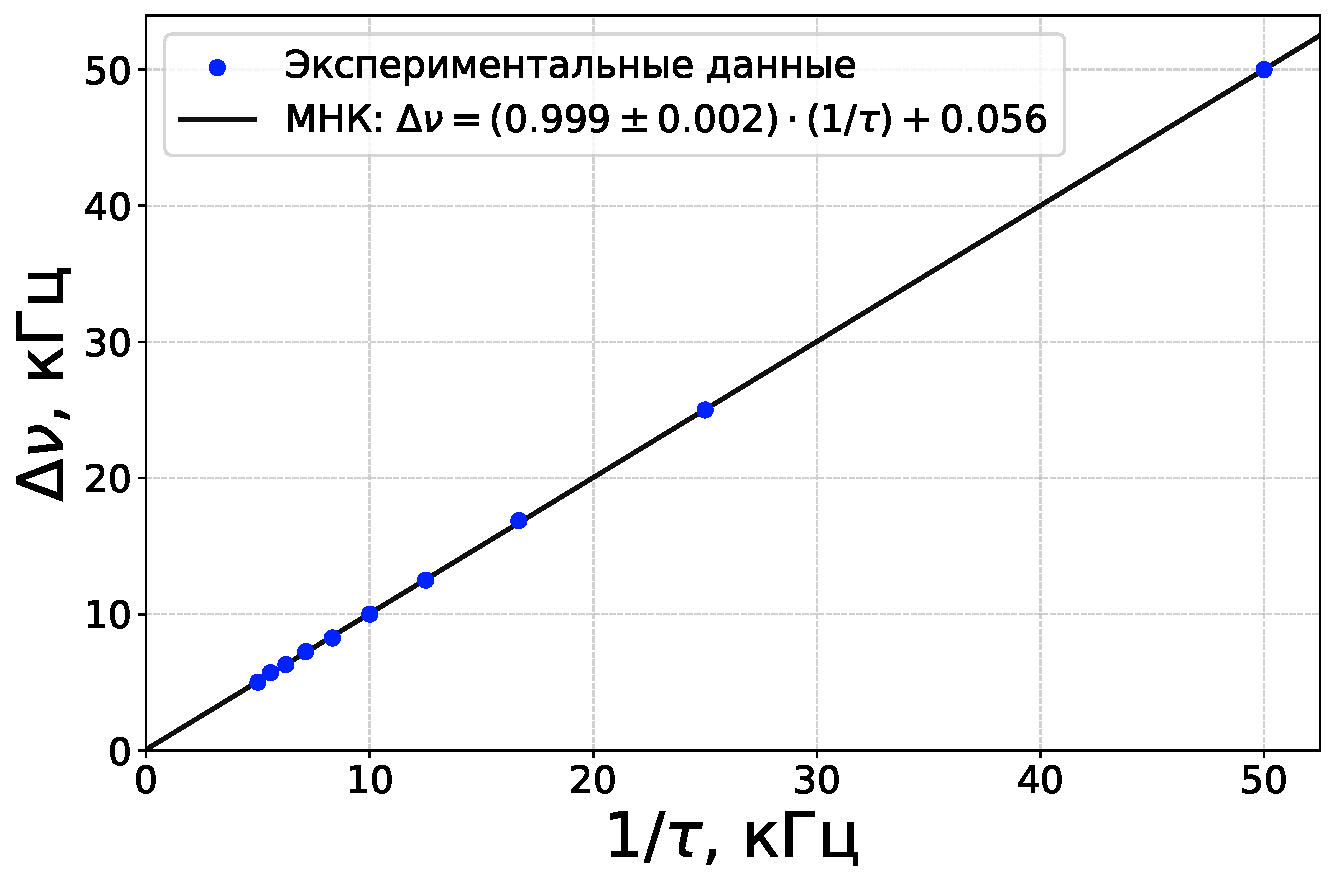
\includegraphics[width=\linewidth]{graph_width_tau.pdf}
        \vspace{-0.8em}
        
        \small а) Зависимость $\Delta\nu$ от $1/\tau$
    \end{minipage}\hfill
    \begin{minipage}{0.48\textwidth}
        \centering
        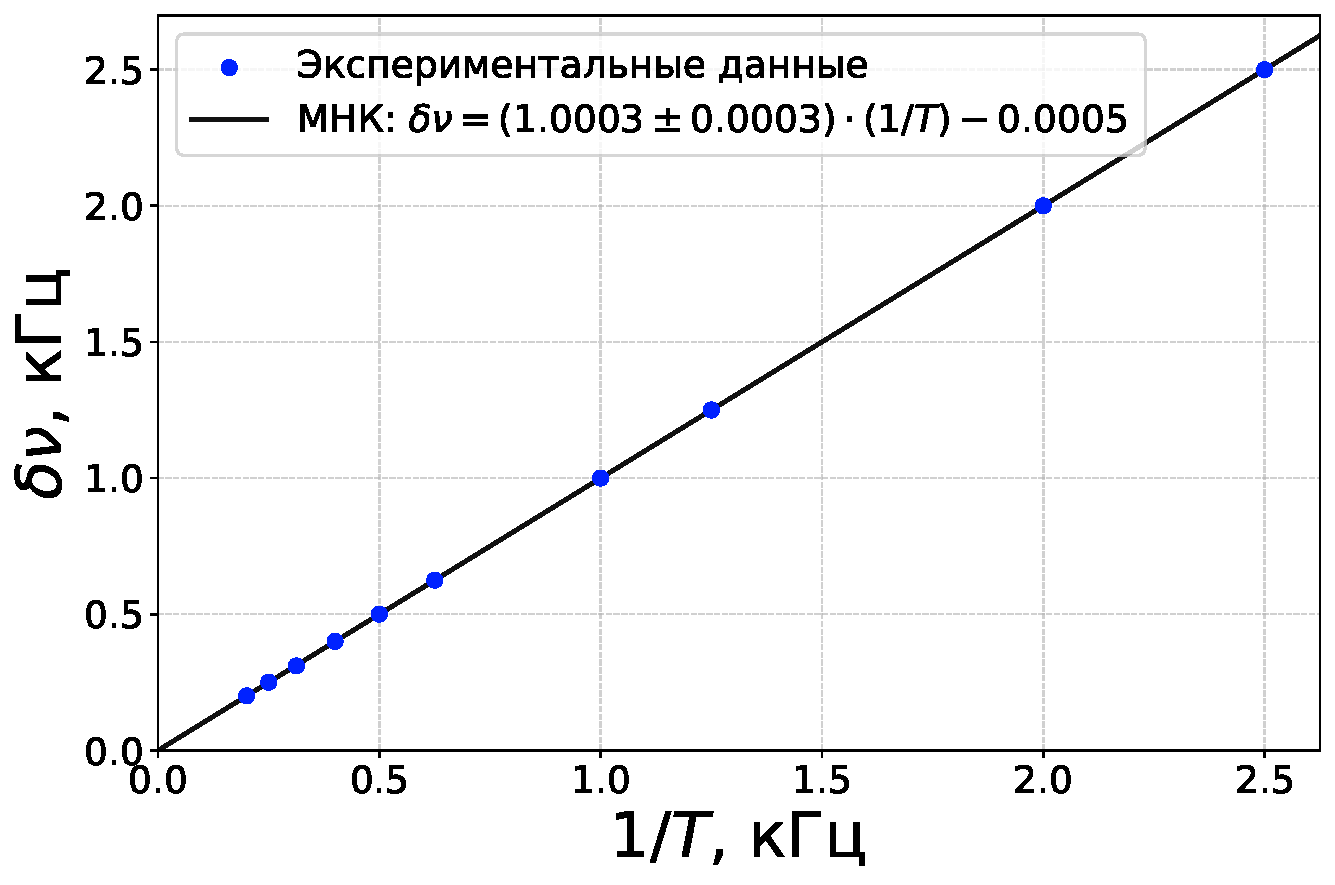
\includegraphics[width=\linewidth]{graph_dist_T.pdf}
        \vspace{-0.8em}
        
        \small б) Зависимость $\delta\nu$ от $1/T$
    \end{minipage}
    \caption{Графики проверки соотношений неопределенностей: (а) для полной ширины спектра импульса; (б) для расстояния между гармониками периодического сигнала.}
    \label{fig:uncertainty_graphs}
\end{figure*}

По полученным экспериментальным точкам были проведены наилучшие прямые с использованием метода наименьших квадратов (МНК) (рис. \ref{fig:uncertainty_graphs}). Погрешности измерений не превышают размеров маркеров, поэтому кресты погрешностей на графиках не отображаются. Зависимость ширины спектра $\Delta\nu$ от обратной длительности импульса $1/\tau$ носит четкий линейный характер, при этом угловой коэффициент аппроксимирующей прямой равен $k_1 = 1.00 \pm 0.02$. Это хорошо согласуется с теоретическими ожиданиями. Аналогично, зависимость расстояния между соседними гармониками $\delta\nu$ от обратного периода $1/T$ также оказалась строго линейной с угловым коэффициентом $k_2 = 1.0003 \pm 0.0003$. Выявленная прямая пропорциональность надежно подтверждает справедливость соотношений неопределенностей для прямоугольных импульсов.

\subsection{Наблюдение спектра периодической последовательности цугов}

Во второй части работы исследовался спектр периодической последовательности цугов — радиоимпульсов с синусоидальным заполнением. На генераторе были установлены следующие исходные параметры сигнала: частота несущей $\nu_0 = 50$ кГц, период повторения $T = 1$ мс (частота повторения $\nu_{\text{повт}} = 1$ кГц) и число периодов синусоиды в одном импульсе $N = 5$. Эффективная длительность такого импульса составила $\tau = N/\nu_0 = 100$ мкс.

Зафиксированные на осциллографе спектрограммы (рис. \ref{fig:burst_spectra}) показывают, что в отличие от прямоугольных импульсов, спектр цугов формируется вокруг частоты высокочастотного заполнения. По сути, огибающая спектра цугов имеет вид функции, аналогичной спектру прямоугольного импульса длительностью $\tau$, но сдвинутой по оси частот и отцентрированной на частоте несущей $\nu_0$.

\begin{figure*}[t!]
    \centering
    \begin{minipage}{0.48\textwidth}
        \centering
        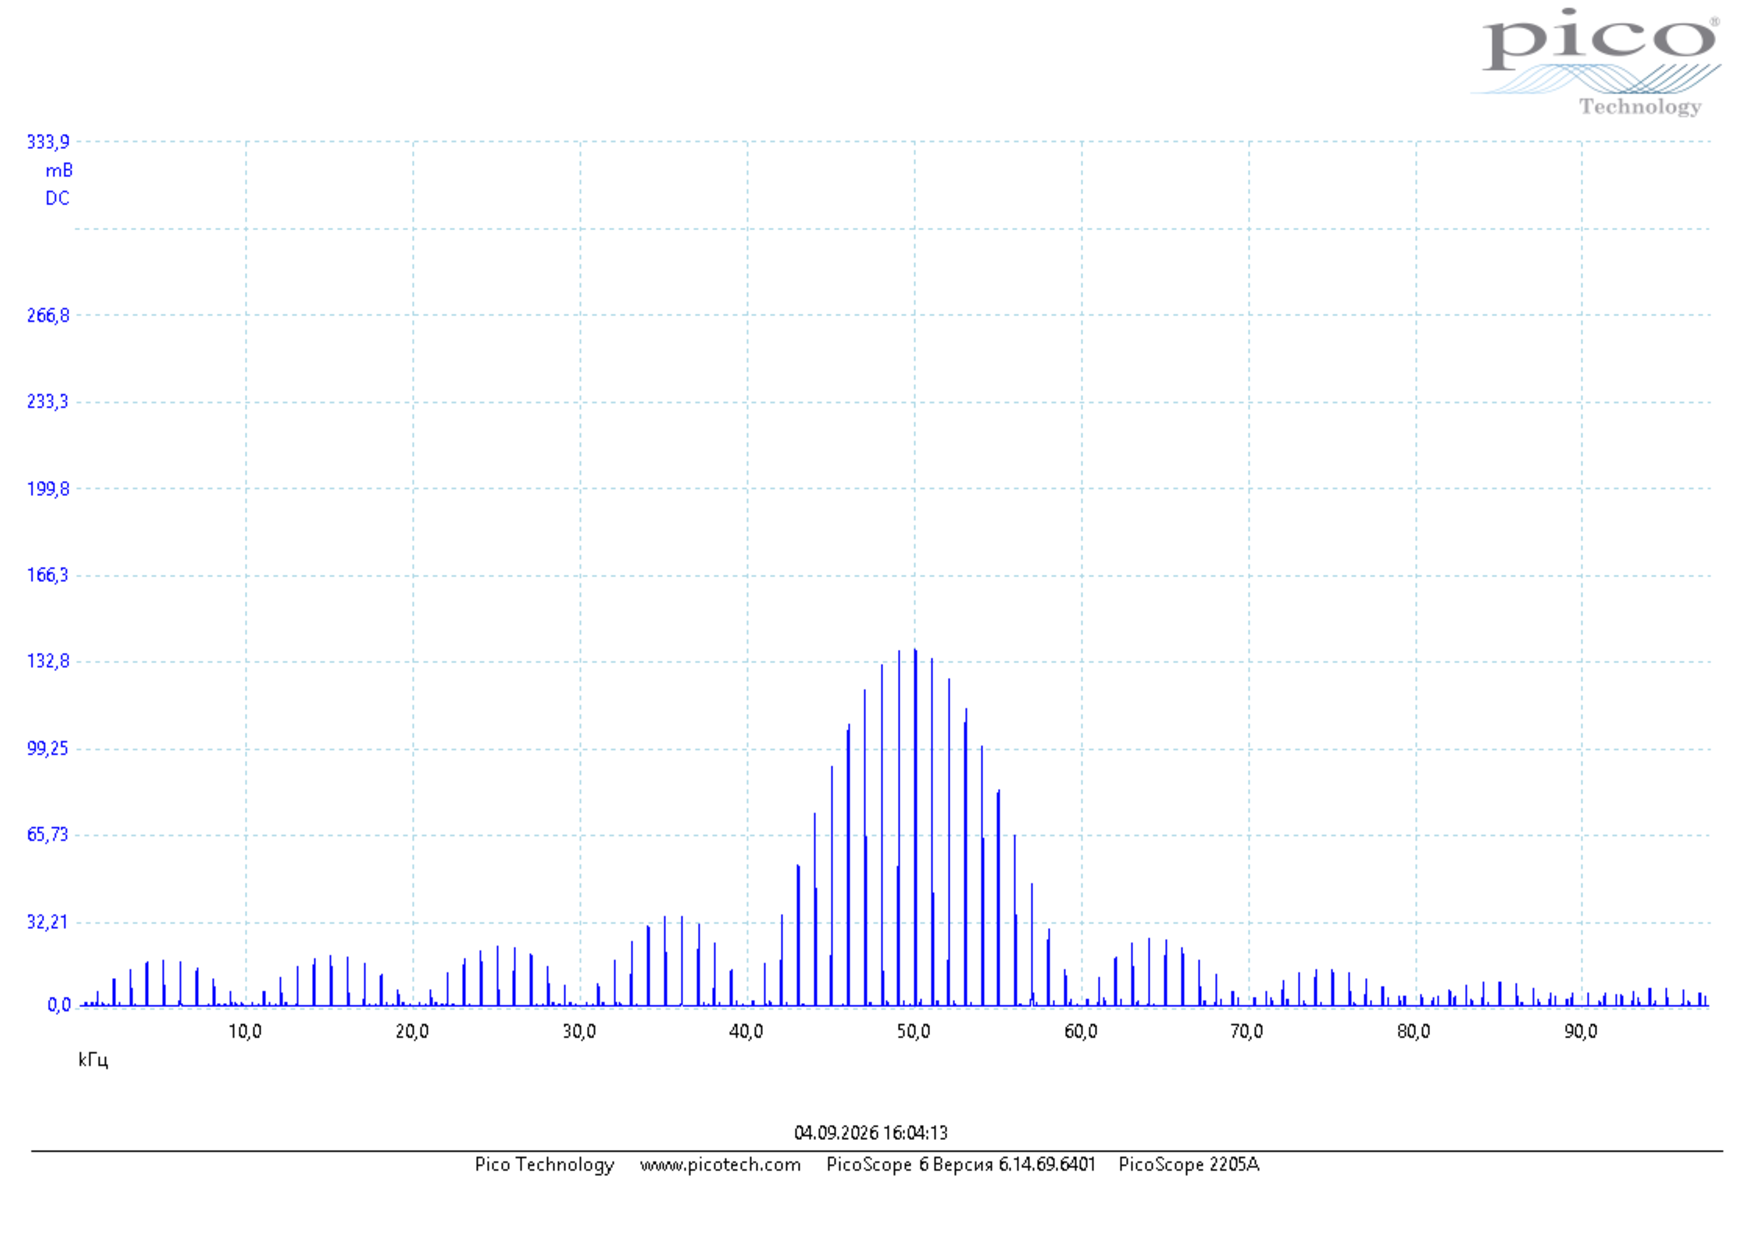
\includegraphics[width=\linewidth]{50kHz_1ms_5cyc.pdf}
        \vspace{-0.8em}
        
        \small а) $\nu_0 = 50$ кГц, $T = 1$ мс, $N = 5$ (исходный)
        \vspace{4mm}
    \end{minipage}\hfill
    \begin{minipage}{0.48\textwidth}
        \centering
        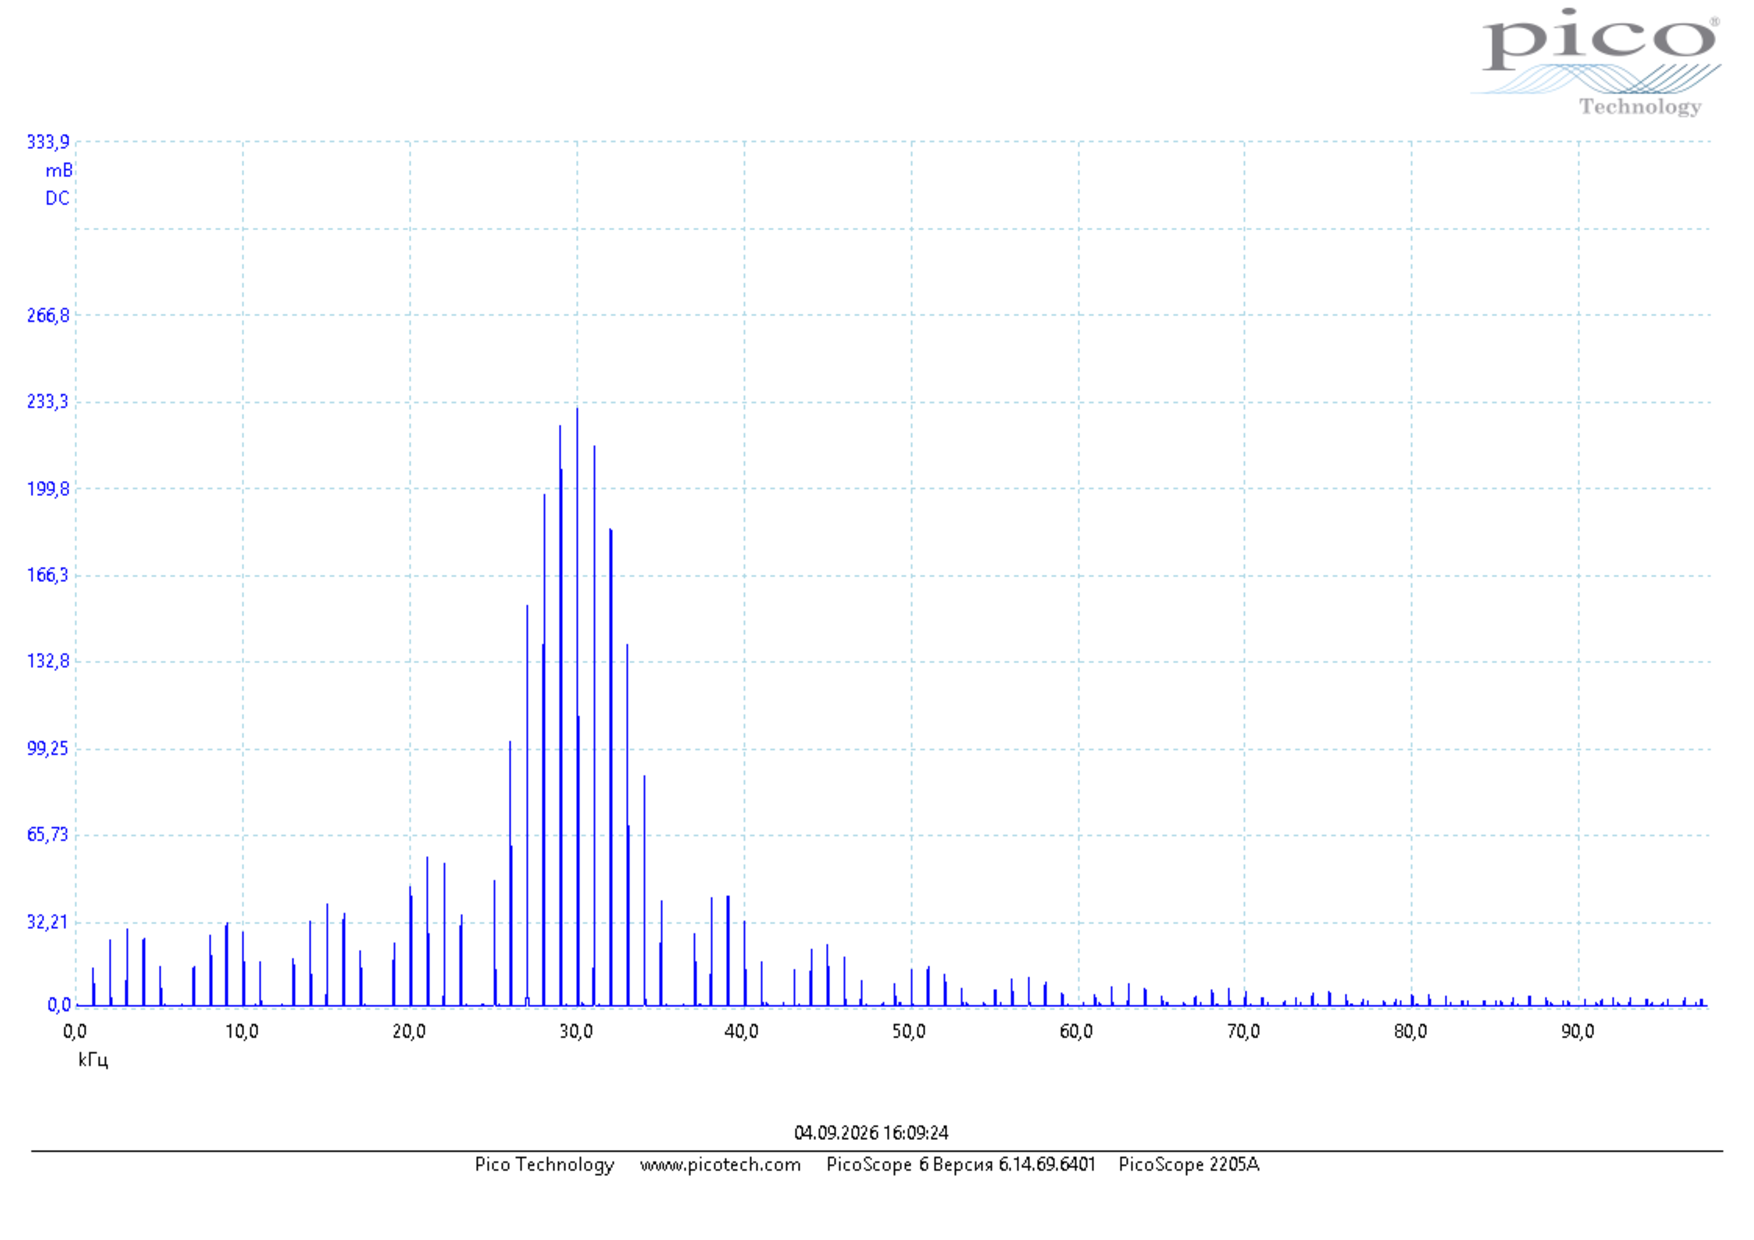
\includegraphics[width=\linewidth]{30kHz_1ms_5cyc.pdf}
        \vspace{-0.8em}
        
        \small б) $\nu_0 = 30$ кГц, $T = 1$ мс, $N = 5$
        \vspace{4mm}
    \end{minipage}
    
    \begin{minipage}{0.48\textwidth}
        \centering
        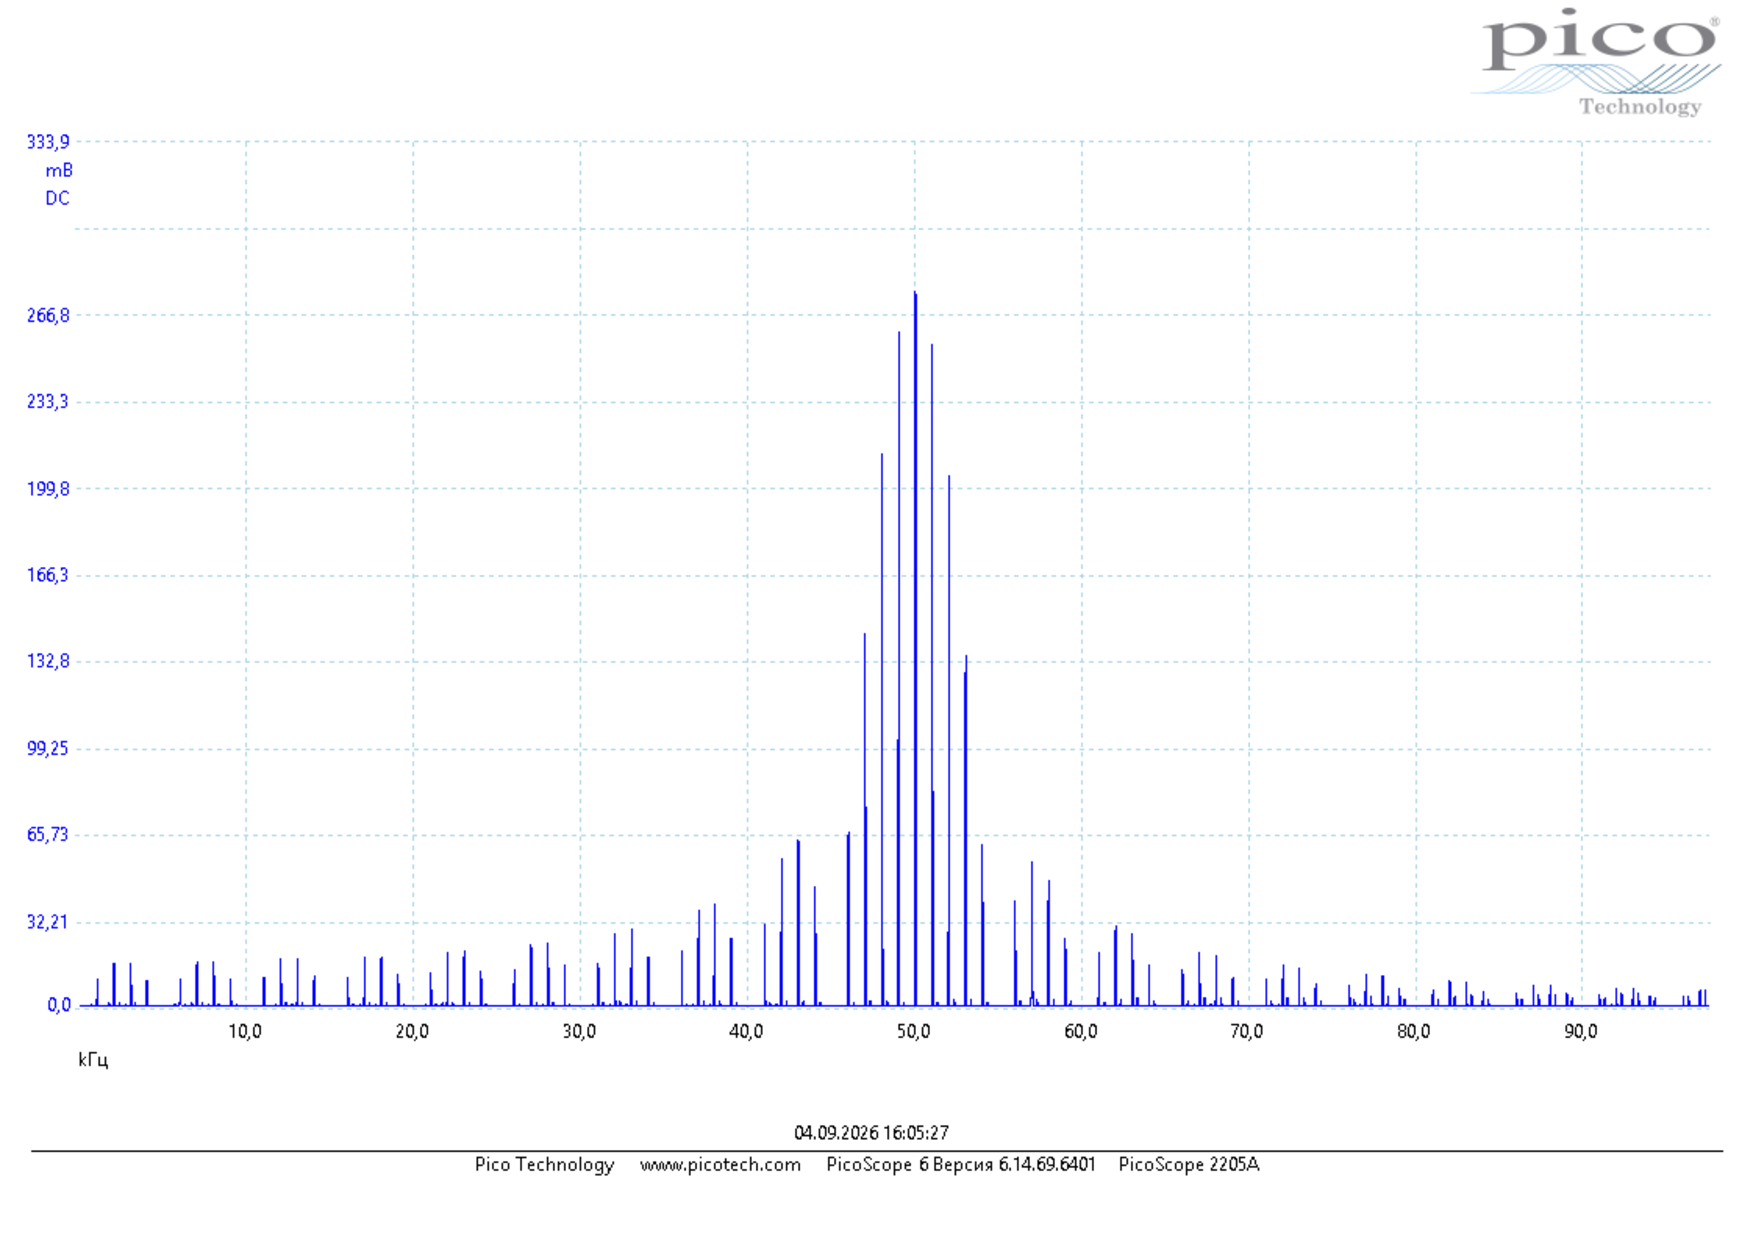
\includegraphics[width=\linewidth]{50kHz_1ms_10cyc.pdf}
        \vspace{-0.8em}
        
        \small в) $\nu_0 = 50$ кГц, $T = 1$ мс, $N = 10$
    \end{minipage}\hfill
    \begin{minipage}{0.48\textwidth}
        \centering
        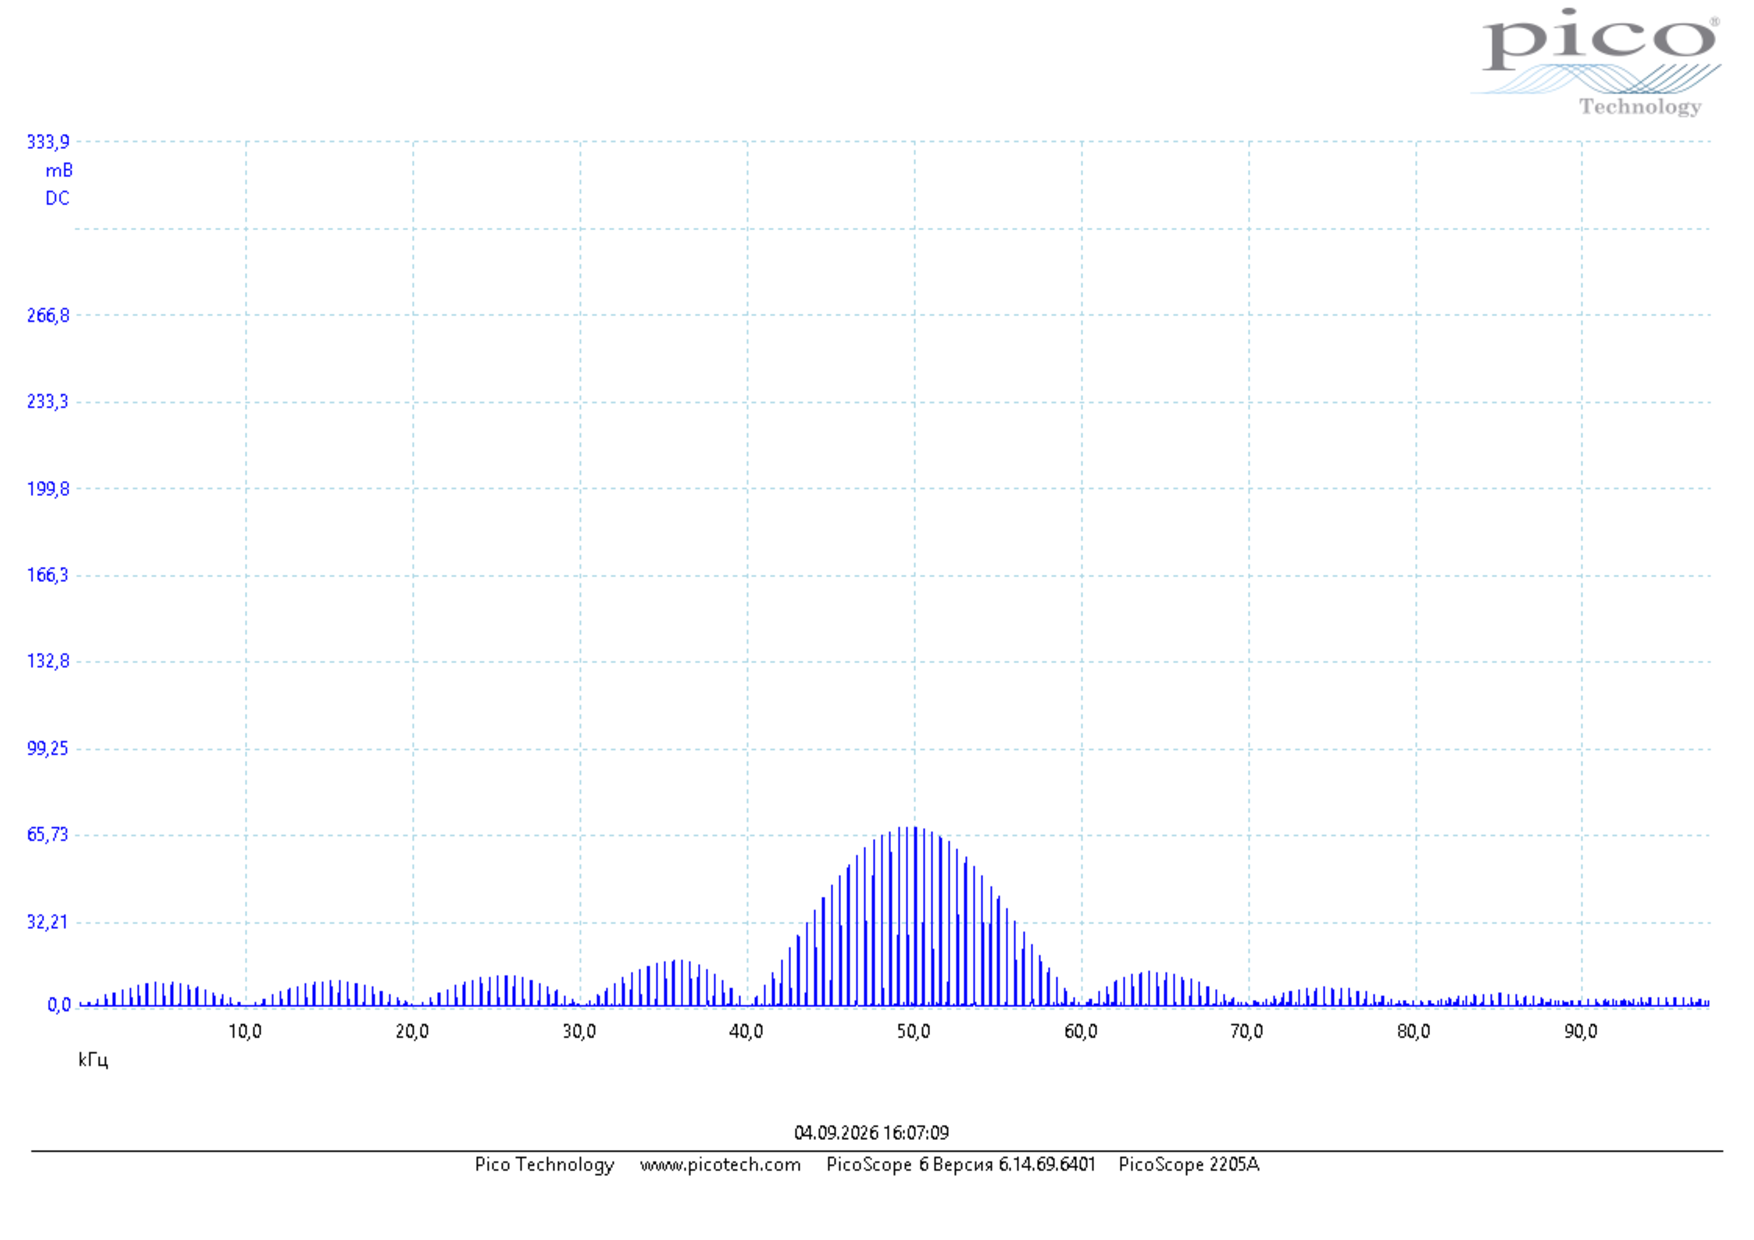
\includegraphics[width=\linewidth]{50kHz_2ms_5cyc.pdf}
        \vspace{-0.8em}
        
        \small г) $\nu_0 = 50$ кГц, $T = 2$ мс, $N = 5$
    \end{minipage}
    \caption{Спектры периодической последовательности цугов при различных параметрах генерации. Центральная частота главного лепестка огибающей строго совпадает с частотой несущей $\nu_0$.}
    \label{fig:burst_spectra}
\end{figure*}

Из полученных спектров хорошо видно, как параметры сигнала влияют на его частотное представление. Уменьшение частоты заполнения с 50 кГц до 30 кГц (рис. \ref{fig:burst_spectra}а и \ref{fig:burst_spectra}б) приводит к эквивалентному смещению всего спектра влево по оси частот. При этом ширина огибающей ожидаемо меняется обратно пропорционально, поскольку увеличивается длительность импульса $\tau = N/\nu_0$. Если же увеличить число периодов $N$ с 5 до 10 при фиксированной $\nu_0$, длительность импульса возрастает в два раза. Как и предсказывает соотношение неопределенностей, это вызывает двукратное сужение главного лепестка огибающей (сравнение рис. \ref{fig:burst_spectra}а и \ref{fig:burst_spectra}в). Наконец, увеличение периода повторения $T$ до 2 мс (рис. \ref{fig:burst_spectra}г) вдвое снижает частоту следования импульсов, из-за чего пропорционально сокращается расстояние между гармониками ($\delta\nu = 1/T$), спектр уплотняется.

\begin{table}[ht!]
    \caption{Параметры спектра периодической последовательности цугов при изменении характеристик генерации. Погрешность курсорных измерений частот не превышает $\pm 0.3$ кГц.}
    \label{tab:burst_params}
    \centering
    \begin{ruledtabular}
    \begin{tabular}{cccccc}
        $\nu_0$, кГц & $T$, мс & $N$ & Центр спектра, кГц & $\Delta\nu$, кГц & $\delta\nu$, кГц \\
        \hline
        30.0 & 1.0 & 5  & $30.0 \pm 0.3$ & $12.0 \pm 0.3$ & $1.00 \pm 0.03$ \\
        50.0 & 1.0 & 5  & $50.0 \pm 0.3$ & $20.0 \pm 0.3$ & $1.00 \pm 0.03$ \\
        50.0 & 1.0 & 10 & $50.0 \pm 0.3$ & $10.0 \pm 0.3$ & $1.00 \pm 0.03$ \\
        50.0 & 2.0 & 5  & $50.0 \pm 0.3$ & $20.0 \pm 0.3$ & $0.50 \pm 0.03$ \\
    \end{tabular}
    \end{ruledtabular}
\end{table}

Данные измерений (табл. \ref{tab:burst_params}) количественно подтверждают описанные наблюдения. Положение центра спектра во всех случаях строго совпало с частотой высокочастотного заполнения $\nu_0$ в пределах погрешности прибора. Это напрямую подтверждает теорему смещения: умножение прямоугольного импульса на гармонический сигнал несущей частоты смещает спектр ровно на величину $\nu_0$. Кроме того, ширина спектра $\Delta\nu$ оказалась обратно пропорциональна эффективной длительности импульса $\tau = N/\nu_0$. Например, при двукратном увеличении числа периодов $N$ ширина спектра сузилась с $20.0 \pm 0.1$ до $10.0 \pm 0.1$ кГц, что удовлетворяет оценке $\Delta\nu \cdot \tau \sim 1$. Расстояние между спектральными линиями $\delta\nu$, как и ожидалось, зависело только от периода повторения $T$. Увеличение $T$ с 1.0 до 2.0 мс закономерно привело к уменьшению $\delta\nu$ в два раза.

\subsection{Исследование спектра амплитудно-модулированного сигнала}

В заключительной части эксперимента изучался гармонический амплитудно-модулированный (АМ) сигнал. На генераторе были установлены следующие начальные параметры: частота несущей $\nu_0 = 50$ кГц, частота модуляции $\nu_{\text{мод}} = 2$ кГц, глубина модуляции $m = 50\%$.

Для проверки заданных параметров сигнала были проведены курсорные измерения амплитуд по осциллограмме. Максимальная и минимальная амплитуды огибающей составили $A_{\text{max}} = 1.47 \pm 0.01$ В и $A_{\text{min}} = 0.488 \pm 0.005$ В соответственно. Расчетная глубина модуляции, вычисленная по экспериментальным данным, составила:
\begin{equation}
    m = \frac{A_{\text{max}} - A_{\text{min}}}{A_{\text{max}} + A_{\text{min}}} = \frac{1.47 - 0.488}{1.47 + 0.488} \approx 0.502.
\end{equation}
С помощью формулы переноса погрешностей косвенных измерений, абсолютная погрешность $\sigma_m$ составила $\pm 0.005$. Следовательно, экспериментально определенная глубина модуляции равна $m = 0.502 \pm 0.005$. Полученное значение совпало с заданным на генераторе значением 50\% с точностью в погрешности.

Далее сигнал анализировался в частотной области. Согласно теории, спектр гармонического АМ-сигнала должен состоять из трех дискретных линий: центральной несущей на частоте $\nu_0$ и двух симметричных боковых гармоник на частотах $\nu_0 - \nu_{\text{мод}}$ и $\nu_0 + \nu_{\text{мод}}$. 

Для проверки расположения спектральных линий была проведена серия измерений при изменении несущей частоты $\nu_0$ и частоты модуляции $\nu_{\text{мод}}$. Измеренные значения частот центральной ($\nu_{\text{осн}}^{\text{эксп}}$) и левой/правой боковых ($\nu_{\text{лев}}^{\text{эксп}}$, $\nu_{\text{прав}}^{\text{эксп}}$) гармоник представлены в табл. \ref{tab:am_freq}. Типичная спектрограмма сигнала представлена на рис. \ref{fig:am_spectra}.

\begin{table}[ht!]
    \caption{Положение спектральных линий АМ-сигнала на оси частот при различных параметрах генерации. Зафиксировано смещение всего спектра в низкочастотную область из-за эффекта алиасинга. Инструментальная погрешность частот составляет $\pm 0.003$ кГц.}
    \label{tab:am_freq}
    \centering
    \begin{ruledtabular}
    \begin{tabular}{ccccc}
        $\nu_0$, кГц & $\nu_{\text{мод}}$, кГц & $\nu_{\text{лев}}^{\text{эксп}}$, кГц & $\nu_{\text{осн}}^{\text{эксп}}$, кГц & $\nu_{\text{прав}}^{\text{эксп}}$, кГц \\
        \hline
        50.0  & 2.0 & 0.826 & 1.173 & 3.173 \\
        100.0 & 2.0 & 0.347 & 2.346 & 4.347 \\
        50.0  & 1.0 & 0.172 & 1.174 & 2.173 \\
    \end{tabular}
    \end{ruledtabular}
\end{table}

\begin{figure}[t!]
    \centering
    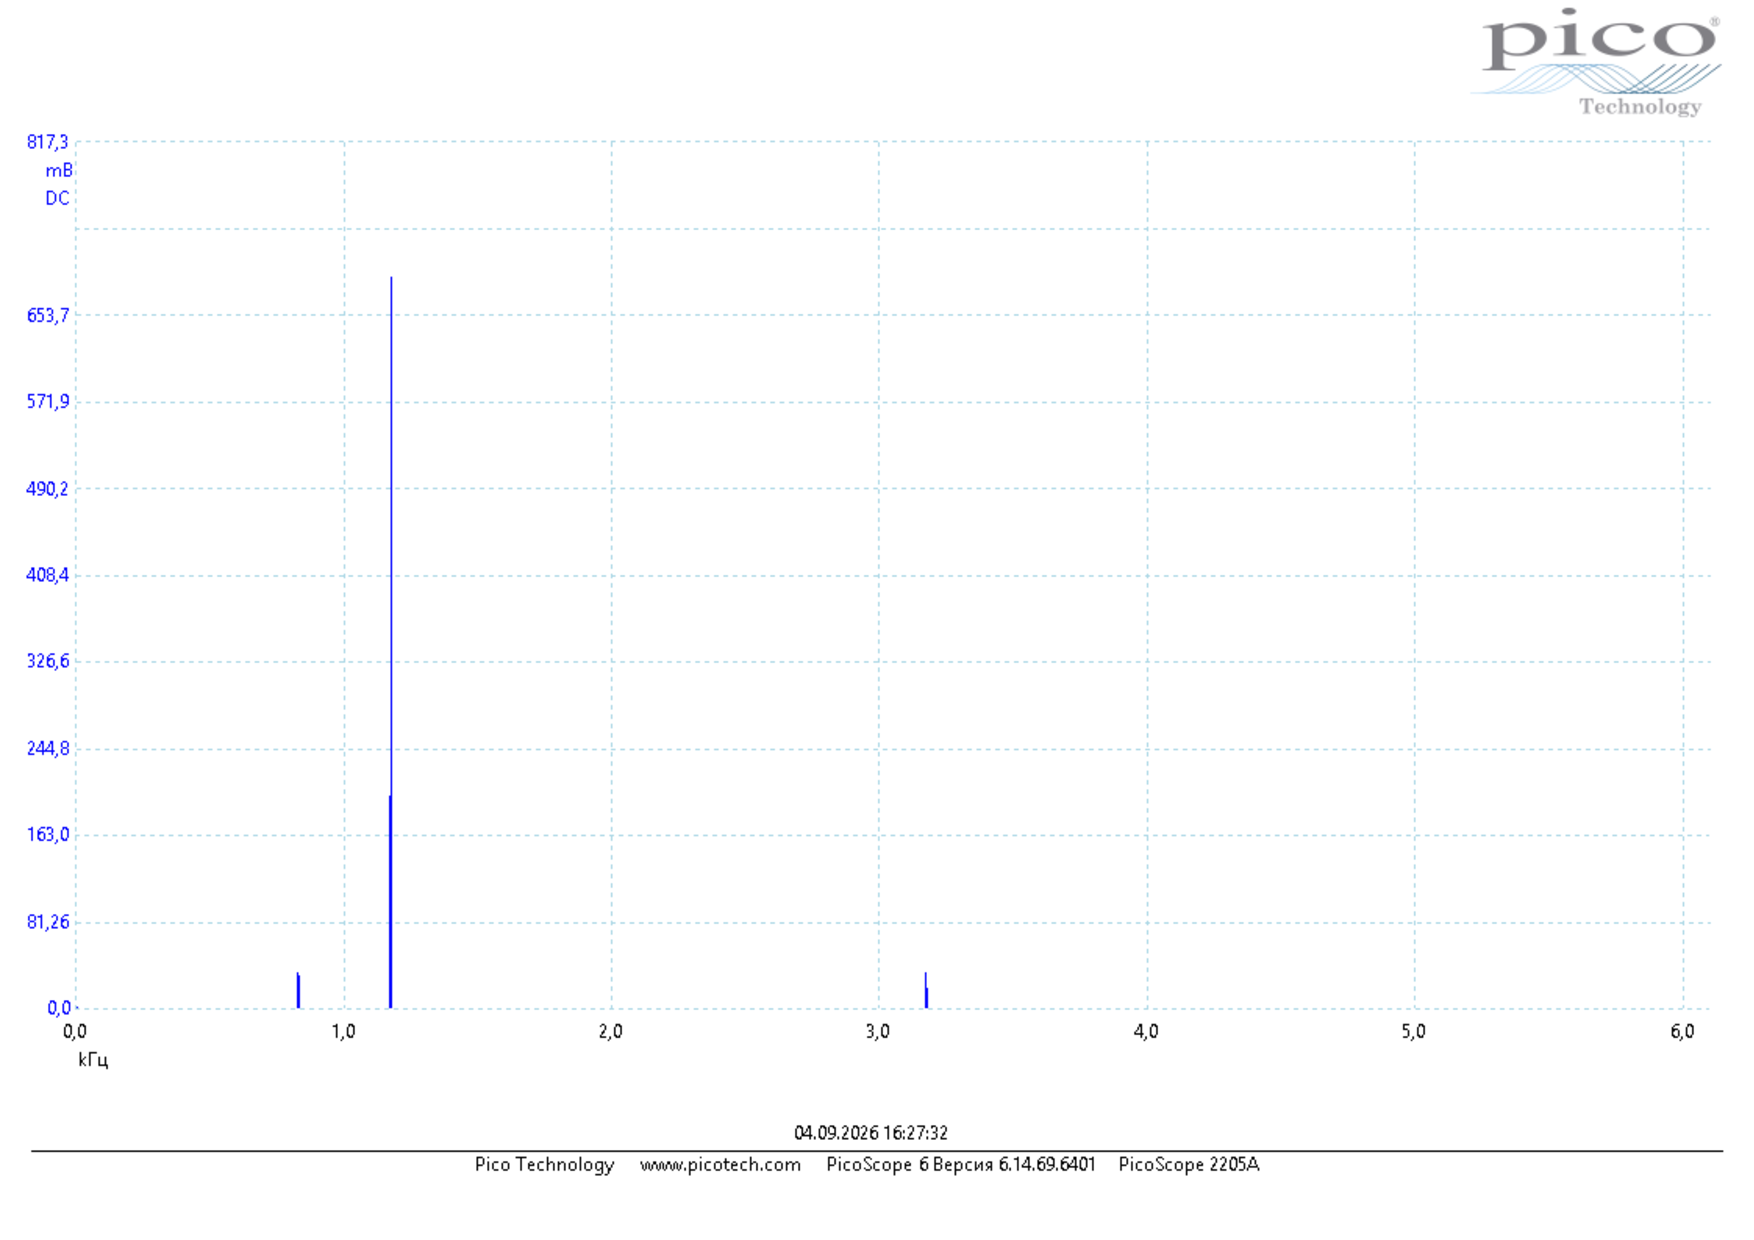
\includegraphics[width=\linewidth]{50kHz_50percent_2kHz.pdf}
    \caption{Спектр амплитудно-модулированного сигнала при несущей частоте 50 кГц, частоте модуляции 2 кГц и глубине модуляции 50\%. Наблюдается смещение спектральной триады из-за аппаратного эффекта наложения спектров.}
    \label{fig:am_spectra}
\end{figure}

При анализе полученных частот был зафиксирован аппаратный эффект наложения спектров (алиасинг). Для визуализации низкочастотной огибающей модуляции (1--2 кГц) временное окно осциллографа было существенно увеличено, что, по-видимому, привело к автоматическому снижению частоты дискретизации в программе PicoScope 6 ниже предела, устанавливаемого теоремой Котельникова. В результате высокочастотные несущие сигналы «свернулись» в низкочастотную область: несущая 50 кГц зафиксировалась на отметке около 1.17 кГц, а несущая 100 кГц — на отметке около 2.35 кГц.

Несмотря на аппаратный сдвиг центральной частоты, фундаментальные свойства АМ-сигнала полностью сохранились. Интервал между центральной и боковыми спектральными линиями остался строго равным установленной частоте модуляции $\nu_{\text{мод}}$. Появление левой боковой гармоники на кажущихся аномальными частотах объясняется отражением спектра от нулевой частоты. Так, для режима с $\nu_0 = 50$ кГц и $\nu_{\text{мод}} = 2$ кГц расчетная частота левой гармоники составляет $1.173 - 2.000 = -0.827$ кГц, что физически проявляется в виде пика на модуле этой частоты $|-0.827| = 0.827$ кГц. Измеренное экспериментальное значение $0.826 \pm 0.003$ кГц подтверждает этот расчет в пределах погрешности. Аналогичное наблюдается для всех остальных наборов параметров генерации.

Помимо частотных характеристик, теоретически регламентируется амплитудный состав АМ-сигнала: отношение амплитуды боковой гармоники к основной должно подчиняться закону $a_{\text{бок}}/a_{\text{осн}} = m/2$. 

Для детальной проверки этого соотношения была проведена серия измерений. На генераторе изменялся коэффициент модуляции $m$ в диапазоне от 10\% до 100\%, и для каждого значения измерялись амплитуды основной $a_{\text{осн}}$ и боковой $a_{\text{бок}}$ спектральных линий. Результаты представлены в табл. \ref{tab:mod_depth}. Амплитуда несущей гармоники во всем диапазоне оставалась неизменной.

\begin{table}[ht!]
    \caption{Зависимость отношения амплитуд спектральных линий от глубины модуляции $m$. Амплитуды измерены с точностью $\pm 0.3$ мВ, инструментальная погрешность отношения $a_{\text{бок}}/a_{\text{осн}}$ рассчитана по формуле косвенных измерений и составляет $\pm 0.001$.}
    \label{tab:mod_depth}
    \centering
    \begin{ruledtabular}
    \begin{tabular}{cccc}
        $m$, \% & $a_{\text{бок}}$, мВ & $a_{\text{осн}}$, мВ & $a_{\text{бок}}/a_{\text{осн}}$ \\
        \hline
        10  & $33.8 \pm 0.3$  & $688.7 \pm 0.3$ & $0.049 \pm 0.001$ \\
        20  & $71.5 \pm 0.3$  & $688.7 \pm 0.3$ & $0.104 \pm 0.001$ \\
        40  & $136.9 \pm 0.3$ & $688.7 \pm 0.3$ & $0.199 \pm 0.001$ \\
        60  & $206.7 \pm 0.3$ & $688.7 \pm 0.3$ & $0.300 \pm 0.001$ \\
        80  & $276.5 \pm 0.3$ & $688.7 \pm 0.3$ & $0.401 \pm 0.001$ \\
        100 & $345.0 \pm 0.3$ & $688.7 \pm 0.3$ & $0.501 \pm 0.001$ \\
    \end{tabular}
    \end{ruledtabular}
\end{table}

\begin{figure}[ht!]
    \centering
    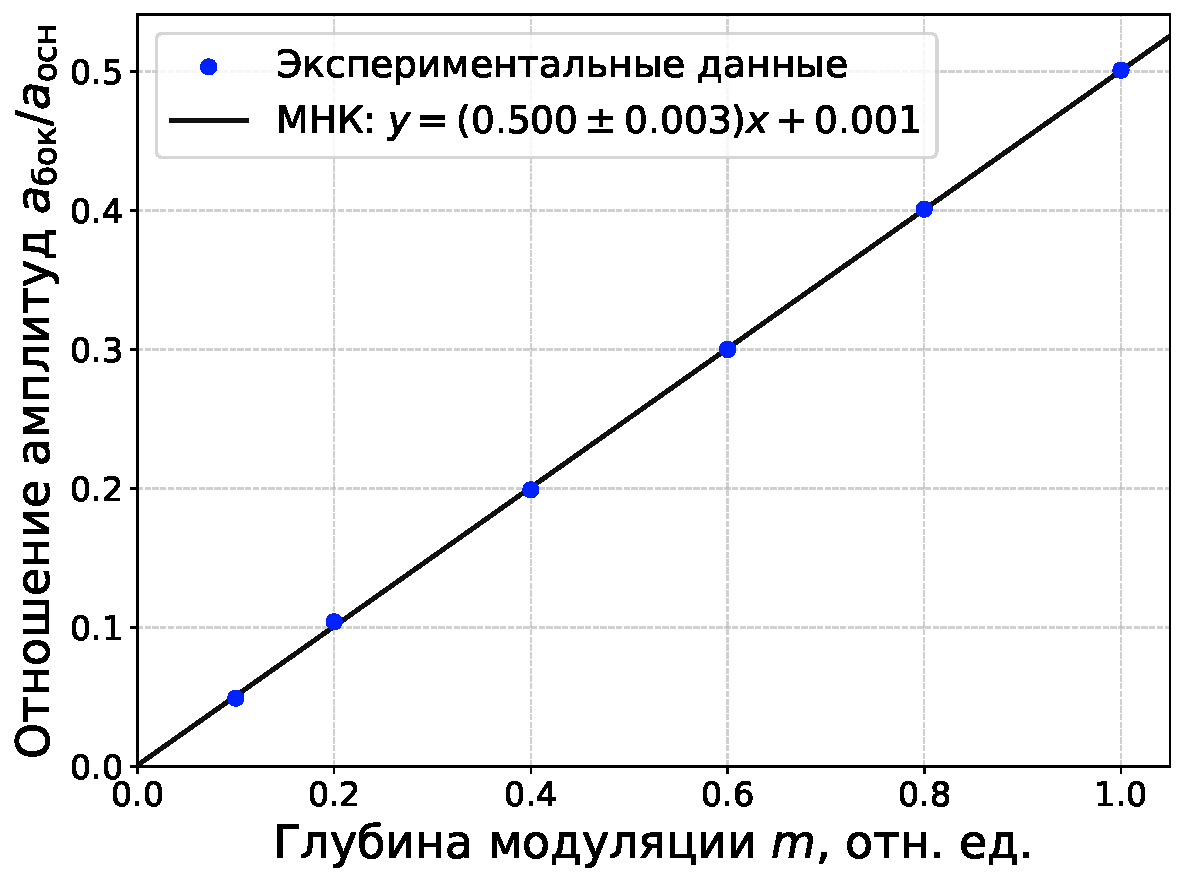
\includegraphics[width=\linewidth]{graph_modulation.pdf}
    \caption{Зависимость отношения амплитуды боковой гармоники к амплитуде основной от глубины модуляции.}
    \label{fig:mod_graph}
\end{figure}

На основе этих данных был построен график зависимости $a_{\text{бок}}/a_{\text{осн}}$ от абсолютного значения глубины модуляции (рис. \ref{fig:mod_graph}). Экспериментальные точки с высокой точностью легли на прямую линию, проходящую через начало координат. Кресты погрешностей на графике не отображены из-за их малости по сравнению с маркерами. Линейная аппроксимация методом наименьших квадратов дала угловой коэффициент $k = 0.501 \pm 0.003$. Полученный результат является экспериментальным подтверждением равенства $a_{\text{бок}}/a_{\text{осн}} = m/2$.

\section{Заключение}

В ходе работы были исследованы спектры различных электрических сигналов методами цифрового Фурье-анализа. Для периодической последовательности прямоугольных импульсов удалось экспериментально подтвердить соотношение неопределенностей: ширина спектральной огибающей действительно обратно пропорциональна длительности импульса ($\Delta\nu \cdot \tau \sim 1$). При этом расстояние между гармониками задается исключительно частотой повторения сигнала ($\delta\nu = 1/T$). Измеренные относительные амплитуды первых восьми гармоник совпали с расчетными значениями с точностью лучше 1.5\%.

Анализ радиоимпульсов с синусоидальным заполнением (цугов) проиллюстрировал теорему смещения. Было показано, что центр огибающей спектра в этом случае располагается на частоте несущей, а ее ширина диктуется эффективной длительностью самого цуга. 

При исследовании амплитудно-модулированного сигнала в спектре наблюдались три компоненты: центральная линия несущей и две симметричные боковые полосы, отстоящие от нее ровно на частоту модуляции. Построенная зависимость отношения амплитуд боковой и основной гармоник от глубины модуляции оказалась линейной. Ее угловой коэффициент составил $0.501 \pm 0.003$, что доказывает теоретическое равенство $a_{\text{бок}}/a_{\text{осн}} = m/2$. В целом, все исследуемые теоретические закономерности спектрального анализа были подтверждены с учетом инструментальных погрешностей.


% --- Библиография ---
\begin{thebibliography}{99}

\bibitem{practicum2019}
Никулин М. Г., Попов П. В. и др. \textit{Лабораторный практикум по общей физике. Том 2. Электричество и магнетизм.} — М.: МФТИ, 2019.

\bibitem{manual361}
\textit{Лабораторная работа 3.6.1 <<Спектральный анализ электрических сигналов>>.} — МФТИ. \href{https://old.mipt.ru/education/chair/physics/S_III/lab_el/3.6.1-2023.pdf}{[Открыть PDF]}

\end{thebibliography}

\end{document}